\chapter{网络中的数据Blob类}
Blob类是Caffe的网络结构中最基本的数据存储类型(可以理解为是对SyncedMemory类型做的一个封装),例如网络权重值和网络的输入、输出等都是以Blob类型进行存储的,因此了解Blob类的内部实现也就成为了解Caffe的基础。
% Section X.1
\section{Blob类的成员}
Blob类是把一块内存空间中存储的数据投影为一个四维矩阵,其中四维矩阵中三维矩阵的数量由num表示,每个三维矩阵中二位矩阵的数量由channels表示(也可以理解为通道数),每个二位矩阵的高和宽由height和width表示。
% Section X.1.1
\subsection{成员变量}
\begin{cntable}{成员变量}{blob/cls/memvar}
  \begin{tabular}{|c|c|l|}
    \hline
    变量名 & 类型 & 功能 \\ \hline
    data\_ & shared\_ptr<SyncedMemory> & 网络链接权重值(指针) \\ \hline
    diff\_ & shared\_ptr<SyncedMemory> & 网络链接的梯度值(指针) \\ \hline
    shape\_data\_ & shared\_ptr<SyncedMemory> & 存储四维矩阵的每个维度值(指针) \\ \hline
    shape\_ & vector<int> & 四维矩阵的每个维度值 \\ \hline
    count\_ & int & 元素的总个数 \\ \hline
    capacity\_ & int & 元素的总个数 \\ \hline
  \end{tabular}
\end{cntable}
这里使用了Boost库中的智能指针shared\_ptr<T>,详细介绍请参考~\ref{deps/boost/ptr}。
% Section X.1.2
\subsection{成员函数}
\subsubsection{构造函数}
Blob类的构造函数有三种重载类型,包括一个无参构造函数、一个多参构造函数和一个含有一个参数的构造函数。值得注意的是,含有多个参数的构造函数已被含有一个参数的构造函数所取代。同时,构造函数前的explicit修饰,代表禁止隐式的类型转换(参考~\ref{c/func/explicit})。三种重载构函数如下所示:

\noindent\ding{47}{\kai{第一种:}}
\begin{minted}{c++}
Blob()
       : data_(), diff_(), count_(0), capacity_(0) {}
\end{minted}

\noindent\ding{47}{\kai{第二种:}}
\begin{minted}{c++}
template <typename Dtype>
Blob<Dtype>::Blob(const int num, const int channels, const int height,
    const int width)
  // capacity_ must be initialized before calling Reshape
  : capacity_(0) {
  Reshape(num, channels, height, width);
}
\end{minted}

\noindent\ding{47}{\kai{第三种:}}
\begin{minted}{c++}
template <typename Dtype>
Blob<Dtype>::Blob(const vector<int>& shape)
  // capacity_ must be initialized before calling Reshape
  : capacity_(0) {
  Reshape(shape);
}
\end{minted}
构造函数调用了另一个成员函数Reshape()。
\subsubsection{Reshape()}
Blob类的Reshape()方法针对不同参数有三种重载类型,如下所示:\\

\noindent\ding{47}{\kai{第一种:}}
\begin{minted}{c++}
template <typename Dtype>
void Blob<Dtype>::Reshape(const vector<int>& shape) {
  CHECK_LE(shape.size(), kMaxBlobAxes);
  count_ = 1;
  shape_.resize(shape.size());
  if (!shape_data_ || shape_data_->size() < shape.size() * sizeof(int)) {
    shape_data_.reset(new SyncedMemory(shape.size() * sizeof(int)));
  }
  int* shape_data = static_cast<int*>(shape_data_->mutable_cpu_data());
  for (int i = 0; i < shape.size(); ++i) {
    CHECK_GE(shape[i], 0);
    if (count_ != 0) {
      CHECK_LE(shape[i], INT_MAX / count_) << "blob size exceeds INT_MAX";
    }
    count_ *= shape[i];
    shape_[i] = shape[i];
    shape_data[i] = shape[i];
  }
  if (count_ > capacity_) {
    
    capacity_ = count_;
    data_.reset(new SyncedMemory(capacity_ * sizeof(Dtype)));
    diff_.reset(new SyncedMemory(capacity_ * sizeof(Dtype)));
  }
}
\end{minted}
该函数的传入参素是Blob数据结构中四维矩阵的四个维度值,函数首先检查维度数不大于最大维度值kMaxBlobAxes,然后设置成员变量shape\_的元素数量,并对成员变量shape\_data\_分配内存。在对shape\_data\_赋值时,首先使用static\_cast进行类型转换(具体参考~\ref{c/type/static}),然后根据函数参数shape对shape\_和shape\_data\_赋值,并计算出元素总数count\_和capacity\_,最后再根据capacity\_来为成员变量data\_和diff\_分配内存。这里注意成员变量shape\_data\_、data\_和diff\_都是指向一个SyncedMemory类型对象的智能指针。\\

\noindent\ding{47}{\kai{第二种:}}
\begin{minted}{c++}
template <typename Dtype>
void Blob<Dtype>::Reshape(const int num, const int channels, const int height,
    const int width) {
  vector<int> shape(4);
  shape[0] = num;
  shape[1] = channels;
  shape[2] = height;
  shape[3] = width;
  Reshape(shape);
}
\end{minted}
不难看出,该重载函数功能是通过内部调用第一种Reshape()函数实现的。\\

\noindent\ding{47}{\kai{第三种:}}
\begin{minted}{c++}
template <typename Dtype>
void Blob<Dtype>::Reshape(const BlobShape& shape) {
  CHECK_LE(shape.dim_size(), kMaxBlobAxes);
  vector<int> shape_vec(shape.dim_size());
  for (int i = 0; i < shape.dim_size(); ++i) {
    shape_vec[i] = shape.dim(i);
  }
  Reshape(shape_vec);
}
\end{minted}
事实上,该函数内部也是调用了第一种Reshape()函数。这里值得注意的是函数的参数类型为BlobShape,该类型的定义实在头文件caffe/proto/caffe.pb.h中,具体可以参考~\ref{deps/protobuf}。
\subsubsection{ReshapeLike()}
该函数通过一个已知的Blob对象来初始化一个新的Blob对象的四维矩阵各个维度值。
\begin{minted}{c++}
template <typename Dtype>
void Blob<Dtype>::ReshapeLike(const Blob<Dtype>& other) {
  Reshape(other.shape());
}
\end{minted}
函数的传入参数为一个Blob对象的引用,通过调用对象的shape()方法返回各个维度的数值,并用这些数值初始化一个新的Blob对象四维矩阵维度。
\subsubsection{gpu\_shape()}
该函数主要对成员变量shape\_data\_进行操作,用来获取其在设备端的数据指针。由于成员变量shape\_data\_为shared\_ptr<SyncedMemory>类型,因此其指向的数据可以位于主机和设备端,存储内容为Blob数据中四维矩阵的每个维度的数值。注意,该函数为常函数,因此不能修改类中的成员变量。
\begin{minted}{c++}
template <typename Dtype>
const int* Blob<Dtype>::gpu_shape() const {
  CHECK(shape_data_);
  return (const int*)shape_data_->gpu_data();
}
\end{minted}
\subsubsection{set\_cpu\_data()}
该函数传入参数为数据指针,完成对Blob类data\_变量的赋值功能。data\_变量为shared\_ptr<SyncedMemory>类型,该赋值功能只是修改了指针指向,但是没有完成内存拷贝。
\begin{minted}{c++}
template <typename Dtype>
void Blob<Dtype>::set_cpu_data(Dtype* data) {
  CHECK(data);
  data_->set_cpu_data(data);
}
\end{minted}
% Section X.1.2
\subsection{获得常数据指针}
\subsubsection{cpu\_data()}
该函数返回Blob对象成员变量data\_在主机端的数据指针。该指针指向一个常数据类型,因此不能通过返回的指针修改数据内容。
\begin{minted}{c++}
template <typename Dtype>
const Dtype* Blob<Dtype>::cpu_data() const {
  CHECK(data_);
  return (const Dtype*)data_->cpu_data();
}
\end{minted}
\subsubsection{gpu\_data()}
该函数返回Blob对象成员变量data\_在设备端的数据指针。该指针指向一个常数据类型,因此不能通过返回的指针修改数据内容。
\begin{minted}{c++}
template <typename Dtype>
const Dtype* Blob<Dtype>::gpu_data() const {
  CHECK(data_);
  return (const Dtype*)data_->gpu_data();
}
\end{minted}
\subsubsection{cpu\_diff()}
该函数返回Blob对象成员变量diff\_在主机端的数据指针。该指针指向一个常数据类型,因此不能通过返回的指针修改数据内容。
\begin{minted}{c++}
template <typename Dtype>
const Dtype* Blob<Dtype>::cpu_diff() const {
  CHECK(diff_);
  return (const Dtype*)diff_->cpu_data();
}
\end{minted}
\subsubsection{gpu\_diff()}
该函数返回Blob对象成员变量diff\_在设备端的数据指针。该指针指向一个常数据类型,因此不能通过返回的指针修改数据内容。
\begin{minted}{c++}
template <typename Dtype>
const Dtype* Blob<Dtype>::gpu_diff() const {
  CHECK(diff_);
  return (const Dtype*)diff_->gpu_data();
}
\end{minted}
% Section X.1.3
\subsection{获得普通数据指针}
\subsubsection{mutabel\_cpu\_data()}
该函数返回Blob对象成员变量data\_在主机端的数据指针。该指针为普通指针,因此可以通过返回的指针修改数据内容。
\begin{minted}{c++}
template <typename Dtype>
Dtype* Blob<Dtype>::mutable_cpu_data() {
  CHECK(data_);
  return static_cast<Dtype*>(data_->mutable_cpu_data());
}
\end{minted}
\subsubsection{mutable\_gpu\_data()}
该函数返回Blob对象成员变量data\_在设备端的数据指针。该指针为普通指针,因此可以通过返回的指针修改数据内容。
\begin{minted}{c++}
template <typename Dtype>
Dtype* Blob<Dtype>::mutable_gpu_data() {
  CHECK(data_);
  return static_cast<Dtype*>(data_->mutable_gpu_data());
}
\end{minted}
\subsubsection{mutable\_cpu\_diff()}
该函数返回Blob对象成员变量diff\_在主机端的数据指针。该指针为普通指针,因此可以通过返回的指针修改数据内容。
\begin{minted}{c++}
template <typename Dtype>
Dtype* Blob<Dtype>::mutable_cpu_diff() {
  CHECK(diff_);
  return static_cast<Dtype*>(diff_->mutable_cpu_data());
}
\end{minted}
\subsubsection{mutable\_gpu\_diff()}
该函数返回Blob对象成员变量diff\_在设备端的数据指针。该指针为普通指针,因此可以通过返回的指针修改数据内容。
\begin{minted}{c++}
template <typename Dtype>
Dtype* Blob<Dtype>::mutable_gpu_diff() {
  CHECK(diff_);
  return static_cast<Dtype*>(diff_->mutable_gpu_data());
}
\end{minted}
% Section X.1.4
\subsection{通过其它Blob对象赋值}
\subsubsection{ShareData()}
该函数的传入参数为另一Blob类型的对象other,函数首先比较两个Blob对象的成员变量count\_是否一致,目的是判断两个Blob对象中的数据个数是否相等,若相等那么使本Blob对象的data\_指针与other的data\_指针指向的同一块数据。
\begin{minted}{c++}
template <typename Dtype>
void Blob<Dtype>::ShareData(const Blob& other) {
  CHECK_EQ(count_, other.count());
  data_ = other.data();
}
\end{minted}
\subsubsection{ShareDiff()}
该函数的传入参数为另一Blob类型的对象other,函数首先比较两个Blob对象的成员变量count\_是否一致,目的是判断两个Blob对象中的数据个数是否相等,若相等那么使本Blob对象的diff\_指针与other的diff\_指针指向的同一块数据。
\begin{minted}{c++}
template <typename Dtype>
void Blob<Dtype>::ShareDiff(const Blob& other) {
  CHECK_EQ(count_, other.count());
  diff_ = other.diff();
}
\end{minted}
% Section X.1.5
\subsection{Blob类内数据运算}
在Blob类内,用来存储数据的成员变量主要有data\_和diff\_,Blob类内同样定义了一些针对这些数据的运算函数。
\subsubsection{Update()}
Update()函数使用diff\_内的数据来更新data\_内的数据,其意义是神经网络中连接权重的更新过程。
\begin{minted}{c++}
template <> void Blob<unsigned int>::Update() { NOT_IMPLEMENTED; }
template <> void Blob<int>::Update() { NOT_IMPLEMENTED; }

template <typename Dtype>
void Blob<Dtype>::Update() {
  // We will perform update based on where the data is located.
  switch (data_->head()) {
  case SyncedMemory::HEAD_AT_CPU:
    // perform computation on CPU
    caffe_axpy<Dtype>(count_, Dtype(-1),
        static_cast<const Dtype*>(diff_->cpu_data()),
        static_cast<Dtype*>(data_->mutable_cpu_data()));
    break;
  case SyncedMemory::HEAD_AT_GPU:
  case SyncedMemory::SYNCED:
#ifndef CPU_ONLY
    // perform computation on GPU
    caffe_gpu_axpy<Dtype>(count_, Dtype(-1),
        static_cast<const Dtype*>(diff_->gpu_data()),
        static_cast<Dtype*>(data_->mutable_gpu_data()));
#else
    NO_GPU;
#endif
    break;
  default:
    LOG(FATAL) << "Syncedmem not initialized.";
  }
}
\end{minted}
其中前两行代码是为了避免模板函数中对于unsigned int和int类型的模板函数的定义(因为Update()方法只针对float和double类型),在函数的实现中使用了NOT\_IMPLEMENTED宏(参考\ref{common/macro/notimpl})。在Update()函数正常定义中,函数首相判断数据所处位置,如果在主机端便调用caffe\_axpy()函数(参考\ref{math/cpu/alg}),如果在设备端则调用caffe\_gpu\_axpy()函数(参考\ref{math/gpu/alg}),具体计算过程如下公式所示:
$$
data[i] = data[i] + (-1) * diff[i]
$$
\subsubsection{asum\_data()}
asum\_data()函数用来计算data\_内的数据元素的和值。
\begin{minted}{c++}
template <> unsigned int Blob<unsigned int>::asum_data() const {
  NOT_IMPLEMENTED;
  return 0;
}

template <> int Blob<int>::asum_data() const {
  NOT_IMPLEMENTED;
  return 0;
}

template <typename Dtype>
Dtype Blob<Dtype>::asum_data() const {
  if (!data_) { return 0; }
  switch (data_->head()) {
  case SyncedMemory::HEAD_AT_CPU:
    return caffe_cpu_asum(count_, cpu_data());
  case SyncedMemory::HEAD_AT_GPU:
  case SyncedMemory::SYNCED:
#ifndef CPU_ONLY
  {
    Dtype asum;
    caffe_gpu_asum(count_, gpu_data(), &asum);
    return asum;
  }
#else
    NO_GPU;
#endif
  case SyncedMemory::UNINITIALIZED:
    return 0;
  default:
    LOG(FATAL) << "Unknown SyncedMemory head state: " << data_->head();
  }
  return 0;
}
\end{minted}
其中前两行代码是为了避免模板函数中对于unsigned int和int类型的模板函数的定义。在asum\_data()函数定义中,函数首相判断数据所处位置,如果在主机端便调用caffe\_cpu\_asum()函数(参考\ref{math/cpu/alg}),如果在设备端则调用caffe\_gpu\_asum()函数(参考\ref{math/gpu/alg}),具体计算过程如下公式所示:
$$
asum = \sum\limits_{i=1}^{n} data[i]
$$
\subsubsection{asum\_diff()}
asum\_diff()函数用来计算diff\_内的数据元素的和值。
\begin{minted}{c++}
template <> unsigned int Blob<unsigned int>::asum_diff() const {
  NOT_IMPLEMENTED;
  return 0;
}

template <> int Blob<int>::asum_diff() const {
  NOT_IMPLEMENTED;
  return 0;
}

template <typename Dtype>
Dtype Blob<Dtype>::asum_diff() const {
  if (!diff_) { return 0; }
  switch (diff_->head()) {
  case SyncedMemory::HEAD_AT_CPU:
    return caffe_cpu_asum(count_, cpu_diff());
  case SyncedMemory::HEAD_AT_GPU:
  case SyncedMemory::SYNCED:
#ifndef CPU_ONLY
  {
    Dtype asum;
    caffe_gpu_asum(count_, gpu_diff(), &asum);
    return asum;
  }
#else
    NO_GPU;
#endif
  case SyncedMemory::UNINITIALIZED:
    return 0;
  default:
    LOG(FATAL) << "Unknown SyncedMemory head state: " << diff_->head();
  }
  return 0;
}
\end{minted}
该函数与asum\_data()完全一致,只是将计算数据换为成员变量diff\_。计算表达式为:
$$
asum = \sum\limits_{i=1}^{n} diff[i]
$$
\subsubsection{sumsq\_data()}
函数sumsq\_data()用来计算成员变量data\_中各个元素的平方和。
\begin{minted}{c++}
template <> unsigned int Blob<unsigned int>::sumsq_data() const {
  NOT_IMPLEMENTED;
  return 0;
}

template <> int Blob<int>::sumsq_data() const {
  NOT_IMPLEMENTED;
  return 0;
}

template <typename Dtype>
Dtype Blob<Dtype>::sumsq_data() const {
  Dtype sumsq;
  const Dtype* data;
  if (!data_) { return 0; }
  switch (data_->head()) {
  case SyncedMemory::HEAD_AT_CPU:
    data = cpu_data();
    sumsq = caffe_cpu_dot(count_, data, data);
    break;
  case SyncedMemory::HEAD_AT_GPU:
  case SyncedMemory::SYNCED:
#ifndef CPU_ONLY
    data = gpu_data();
    caffe_gpu_dot(count_, data, data, &sumsq);
#else
    NO_GPU;
#endif
    break;
  case SyncedMemory::UNINITIALIZED:
    return 0;
  default:
    LOG(FATAL) << "Unknown SyncedMemory head state: " << data_->head();
  }
  return sumsq;
}
\end{minted}
其中前两行代码是为了避免模板函数中对于unsigned int和int类型的模板函数的定义。在sumsq\_data()函数定义中,函数首先判断数据所处位置,如果在主机端便调用caffe\_cpu\_dot()函数(参考\ref{math/cpu/alg}),如果在设备端则调用caffe\_gpu\_dot()函数(参考\ref{math/gpu/alg}),具体计算过程如下公式所示:
$$
sumsq = \sum\limits_{i=1}^{n} data[i]*data[i]
$$
\subsubsection{sumsq\_diff()}
函数sumsq\_data()用来计算成员变量diff\_中各个元素的平方和。
\begin{minted}{c++}
template <> unsigned int Blob<unsigned int>::sumsq_diff() const {
  NOT_IMPLEMENTED;
  return 0;
}

template <> int Blob<int>::sumsq_diff() const {
  NOT_IMPLEMENTED;
  return 0;
}

template <typename Dtype>
Dtype Blob<Dtype>::sumsq_diff() const {
  Dtype sumsq;
  const Dtype* diff;
  if (!diff_) { return 0; }
  switch (diff_->head()) {
  case SyncedMemory::HEAD_AT_CPU:
    diff = cpu_diff();
    sumsq = caffe_cpu_dot(count_, diff, diff);
    break;
  case SyncedMemory::HEAD_AT_GPU:
  case SyncedMemory::SYNCED:
#ifndef CPU_ONLY
    diff = gpu_diff();
    caffe_gpu_dot(count_, diff, diff, &sumsq);
    break;
#else
    NO_GPU;
#endif
  case SyncedMemory::UNINITIALIZED:
    return 0;
  default:
    LOG(FATAL) << "Unknown SyncedMemory head state: " << data_->head();
  }
  return sumsq;
}
\end{minted}
该函数与sumsq\_data()完全一致,只是将计算数据换为成员变量diff\_。计算表达式为:
$$
sumsq = \sum\limits_{i=1}^{n} diff[i]*diff[i]
$$
\subsubsection{scale\_data()}
该函数对成员变量data\_中的每个元素乘一个常数,进行尺度上的拉伸。
\begin{minted}{c++}
template <> void Blob<unsigned int>::scale_data(unsigned int scale_factor) {
  NOT_IMPLEMENTED;
}

template <> void Blob<int>::scale_data(int scale_factor) {
  NOT_IMPLEMENTED;
}

template <typename Dtype>
void Blob<Dtype>::scale_data(Dtype scale_factor) {
  Dtype* data;
  if (!data_) { return; }
  switch (data_->head()) {
  case SyncedMemory::HEAD_AT_CPU:
    data = mutable_cpu_data();
    caffe_scal(count_, scale_factor, data);
    return;
  case SyncedMemory::HEAD_AT_GPU:
  case SyncedMemory::SYNCED:
#ifndef CPU_ONLY
    data = mutable_gpu_data();
    caffe_gpu_scal(count_, scale_factor, data);
    return;
#else
    NO_GPU;
#endif
  case SyncedMemory::UNINITIALIZED:
    return;
  default:
    LOG(FATAL) << "Unknown SyncedMemory head state: " << data_->head();
  }
}
\end{minted}
其中前两行代码是为了避免模板函数中对于unsigned int和int类型的模板函数的定义。在scale\_data()函数定义中,函数首先判断数据所处位置,如果在主机端便调用caffe\_scal()函数(参考\ref{math/cpu/alg}),如果在设备端则调用caffe\_gpu\_scal()函数(参考\ref{math/gpu/alg}),具体计算过程如下公式所示:
$$
data[i] = scale\_factor * data[i]
$$
\subsubsection{scale\_diff()}
该函数对成员变量diff\_中的每个元素乘一个常数,进行尺度上的拉伸。
\begin{minted}{c++}
template <> void Blob<unsigned int>::scale_diff(unsigned int scale_factor) {
  NOT_IMPLEMENTED;
}

template <> void Blob<int>::scale_diff(int scale_factor) {
  NOT_IMPLEMENTED;
}

template <typename Dtype>
void Blob<Dtype>::scale_diff(Dtype scale_factor) {
  Dtype* diff;
  if (!diff_) { return; }
  switch (diff_->head()) {
  case SyncedMemory::HEAD_AT_CPU:
    diff = mutable_cpu_diff();
    caffe_scal(count_, scale_factor, diff);
    return;
  case SyncedMemory::HEAD_AT_GPU:
  case SyncedMemory::SYNCED:
#ifndef CPU_ONLY
    diff = mutable_gpu_diff();
    caffe_gpu_scal(count_, scale_factor, diff);
    return;
#else
    NO_GPU;
#endif
  case SyncedMemory::UNINITIALIZED:
    return;
  default:
    LOG(FATAL) << "Unknown SyncedMemory head state: " << diff_->head();
  }
}
\end{minted}
该函数与scale\_data()完全一致,只是将计算数据换为成员变量diff\_。计算表达式为:
$$
diff[i] = scale\_factor * diff[i]
$$
\subsubsection{CopyFrom()}
该函数从一个已有的Blob对象中将数据拷贝到当前的Blob对象中。
\begin{minted}{c++}
template <typename Dtype>
void Blob<Dtype>::CopyFrom(const Blob& source, bool copy_diff, bool reshape) {
  if (source.count() != count_ || source.shape() != shape_) {
    if (reshape) {
      ReshapeLike(source);
    } else {
      LOG(FATAL) << "Trying to copy blobs of different sizes.";
    }
  }
  switch (Caffe::mode()) {
  case Caffe::GPU:
    if (copy_diff) {
      caffe_copy(count_, source.gpu_diff(),
          static_cast<Dtype*>(diff_->mutable_gpu_data()));
    } else {
      caffe_copy(count_, source.gpu_data(),
          static_cast<Dtype*>(data_->mutable_gpu_data()));
    }
    break;
  case Caffe::CPU:
    if (copy_diff) {
      caffe_copy(count_, source.cpu_diff(),
          static_cast<Dtype*>(diff_->mutable_cpu_data()));
    } else {
      caffe_copy(count_, source.cpu_data(),
          static_cast<Dtype*>(data_->mutable_cpu_data()));
    }
    break;
  default:
    LOG(FATAL) << "Unknown caffe mode.";
  }
}
\end{minted}
函数首先判断是否要进行reshape操作,目的是使当前Blob对象的存储维度与源Blob一致。然后判断是否对Blob中的diff\_数据进行拷贝。函数内部通过调用caffe\_copy()函数(参考\ref{math/cpu/alg})完成拷贝操作,该拷贝操作为深度拷贝。
% Section X.1.6
\subsection{BlobProto输入输出}
\subsubsection{ShapeEquals()}
该函数比较Blob对象中存储数据的维度信息与传入的BlobProto对象的维度信息是否一致。
\begin{minted}{c++}
template <typename Dtype>
bool Blob<Dtype>::ShapeEquals(const BlobProto& other) {
  if (other.has_num() || other.has_channels() ||
      other.has_height() || other.has_width()) {
    // Using deprecated 4D Blob dimensions --
    // shape is (num, channels, height, width).
    // Note: we do not use the normal Blob::num(), Blob::channels(), etc.
    // methods as these index from the beginning of the blob shape, where legacy
    // parameter blobs were indexed from the end of the blob shape (e.g., bias
    // Blob shape (1 x 1 x 1 x N), IP layer weight Blob shape (1 x 1 x M x N)).
    return shape_.size() <= 4 &&
           LegacyShape(-4) == other.num() &&
           LegacyShape(-3) == other.channels() &&
           LegacyShape(-2) == other.height() &&
           LegacyShape(-1) == other.width();
  }
  vector<int> other_shape(other.shape().dim_size());
  for (int i = 0; i < other.shape().dim_size(); ++i) {
    other_shape[i] = other.shape().dim(i);
  }
  return shape_ == other_shape;
}
\end{minted}
由于在BlobProto中存在两种数据维度描述方式(参考\ref{proto/file/blob}),因此首先进行判断:如果为旧方式,则对每个维度进行比较;如果为新方式,则读取shape中的维度信息存储到vector<int>对象中,然后进行比较。
\subsubsection{FromProto()}
该函数将数据从BlobProto对象中拷贝到当前Blob对象。
\begin{minted}{c++}
template <typename Dtype>
void Blob<Dtype>::FromProto(const BlobProto& proto, bool reshape) {
  if (reshape) {
    vector<int> shape;
    if (proto.has_num() || proto.has_channels() ||
        proto.has_height() || proto.has_width()) {
      // Using deprecated 4D Blob dimensions --
      // shape is (num, channels, height, width).
      shape.resize(4);
      shape[0] = proto.num();
      shape[1] = proto.channels();
      shape[2] = proto.height();
      shape[3] = proto.width();
    } else {
      shape.resize(proto.shape().dim_size());
      for (int i = 0; i < proto.shape().dim_size(); ++i) {
        shape[i] = proto.shape().dim(i);
      }
    }
    Reshape(shape);
  } else {
    CHECK(ShapeEquals(proto)) << "shape mismatch (reshape not set)";
  }
  // copy data
  Dtype* data_vec = mutable_cpu_data();
  if (proto.double_data_size() > 0) {
    CHECK_EQ(count_, proto.double_data_size());
    for (int i = 0; i < count_; ++i) {
      data_vec[i] = proto.double_data(i);
    }
  } else {
    CHECK_EQ(count_, proto.data_size());
    for (int i = 0; i < count_; ++i) {
      data_vec[i] = proto.data(i);
    }
  }
  if (proto.double_diff_size() > 0) {
    CHECK_EQ(count_, proto.double_diff_size());
    Dtype* diff_vec = mutable_cpu_diff();
    for (int i = 0; i < count_; ++i) {
      diff_vec[i] = proto.double_diff(i);
    }
  } else if (proto.diff_size() > 0) {
    CHECK_EQ(count_, proto.diff_size());
    Dtype* diff_vec = mutable_cpu_diff();
    for (int i = 0; i < count_; ++i) {
      diff_vec[i] = proto.diff(i);
    }
  }
}
\end{minted}
函数首先判断是否进行reshape操作,在reshape操作中,如果当前Blob对象与BlobProto对象的数据维度不一致,那么根据BlobProto对象进行reshape。在拷贝中,由于BlobProto对象的数据字段有float和double两种描述类型,因此通过data\_size()和double\_data\_size()方法的返回值是否大于0来判断存储的数据类型,然后进行深度拷贝操作。该拷贝操作包含data\_和diff\_两部分。
\subsubsection{ToProto()}
该函数将当前Blob对象数据保存为BlobProto对象数据。
\begin{minted}{c++}
template <>
void Blob<double>::ToProto(BlobProto* proto, bool write_diff) const {
  proto->clear_shape();
  for (int i = 0; i < shape_.size(); ++i) {
    proto->mutable_shape()->add_dim(shape_[i]);
  }
  proto->clear_double_data();
  proto->clear_double_diff();
  const double* data_vec = cpu_data();
  for (int i = 0; i < count_; ++i) {
    proto->add_double_data(data_vec[i]);
  }
  if (write_diff) {
    const double* diff_vec = cpu_diff();
    for (int i = 0; i < count_; ++i) {
      proto->add_double_diff(diff_vec[i]);
    }
  }
}

template <>
void Blob<float>::ToProto(BlobProto* proto, bool write_diff) const {
  proto->clear_shape();
  for (int i = 0; i < shape_.size(); ++i) {
    proto->mutable_shape()->add_dim(shape_[i]);
  }
  proto->clear_data();
  proto->clear_diff();
  const float* data_vec = cpu_data();
  for (int i = 0; i < count_; ++i) {
    proto->add_data(data_vec[i]);
  }
  if (write_diff) {
    const float* diff_vec = cpu_diff();
    for (int i = 0; i < count_; ++i) {
      proto->add_diff(diff_vec[i]);
    }
  }
}
\end{minted}
首先使用clear\_shape()方法清空BlobProto中的shape字段数据,然后根据当前Blob对象的shape\_成员为其赋值。类似地,通过clear\_double\_data()和clear\_double\_diff()方法清空BlobProto对象的double\_data和double\_diff字段数据,然后根据当前Blob对象的data\_和diff\_成员为其赋值。
% Section X.1.7
\subsection{初始化模板}
\begin{minted}{c++}
INSTANTIATE_CLASS(Blob);
template class Blob<int>;
template class Blob<unsigned int>;
\end{minted}
在Blob类的最后阶段,对Blob类模板进行初始化,通过INSTANTIATE\_CLASS(Blob)宏(参考\ref{common/macro/instantiate})完成float和double类型的初始化,然后再显式进行了int和unsigned int类型的初始化。
% Section X.2
\section{Blob类的结构}
% Section X.2.1
\subsection{类的初始化}
Blob类通过Reshape()函数进行成员数据内存的分配,Reshape()函数根据不同输入参数存在三个重载类型,同时Blob类的构造函数也是通过对Reshape()函数的调用实现的。
\begin{cnfigure}{Blob类的初始化}{blob/architecture/init}
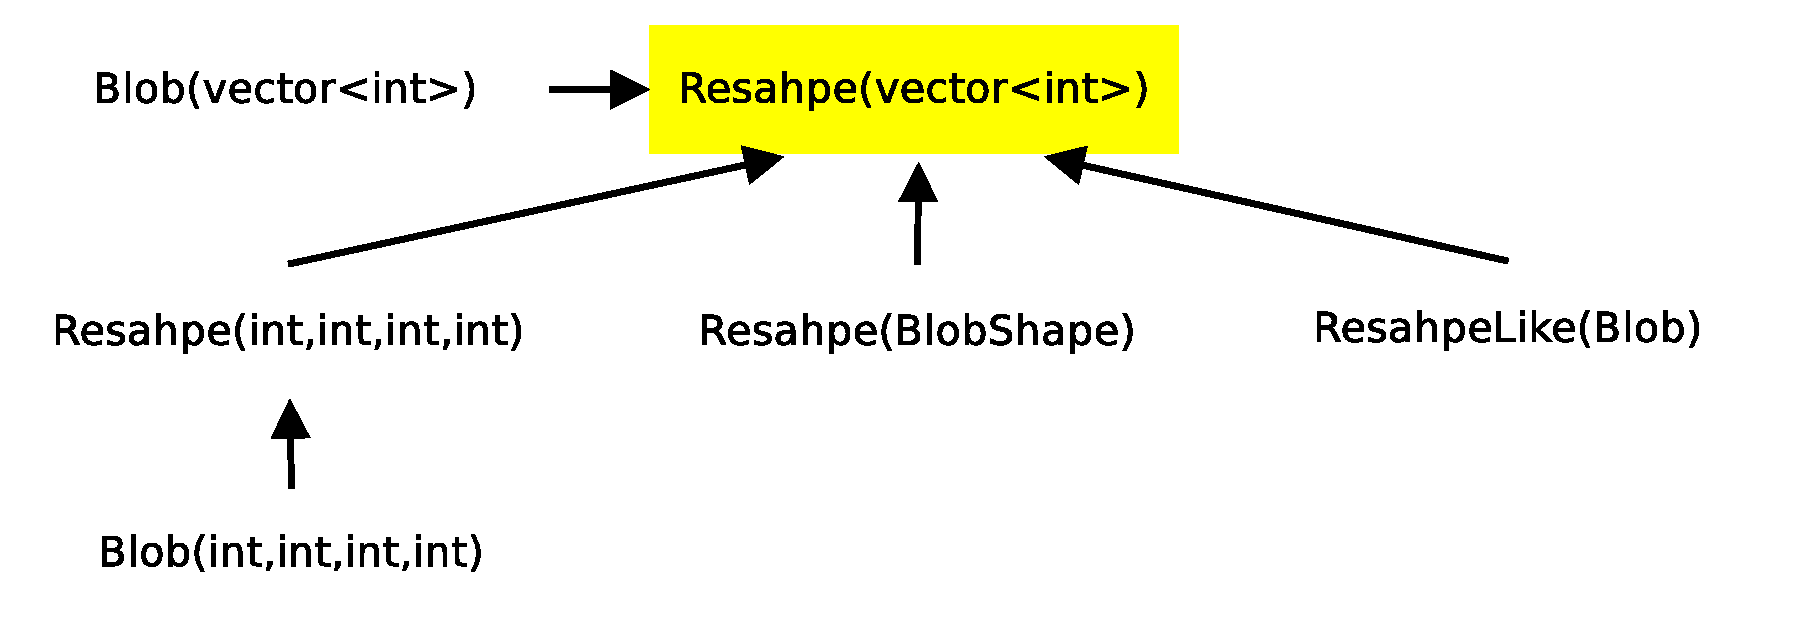
\includegraphics[height=5cm ,width=15cm,angle=0]{include/chp_blob_cls/figures/blob_architecture_reshape.eps}
\end{cnfigure}
% Section X.2.2
\subsection{数据指针的获取}
Blob中维护的数据包括data和diff两部分,内部的数据类型为SyncedMemory。Blob类通过成员函数来获取不同类型的数据指针,从而进行下一步的读取和写入操作。
\begin{cntable}{数据指针获取}{blob/architecture/getptr}
  \begin{tabular}{|l|l|l|l|}
    \hline
          & \makecell[cc]{\hei CPU} & \makecell[cc]{\hei GPU} & \\\hline
    \hei shape &  & gpu\_shape() &  \\ \hline
    \hei data  & \makecell[cl]{cpu\_data() \\ set\_cpu\_data() \\ mutable\_cpu\_data()} & gpu\_data() & shareData() \\ \hline
    \hei diff  & \makecell[cl]{cpu\_diff() \\ mutable\_cpu\_diff()} & \makecell[cl]{gpu\_diff() \\ mutable\_gpu\_diff()} & shareDiff() \\ \hline
  \end{tabular}
\end{cntable}
% Section X.2.3
\subsection{Blob中的数学运算}
Blob类中有一类函数涉及到代数运算操作,在Caffe中几乎所有运算相关操作都是通过内部调用cBLAS或cuBLAS运算库在CPU或GPU上完成的,这部份内容可以参考\ref{math/cpu/alg}和\ref{math/gpu/alg}。
\begin{cntable}{Blob中的数学运算}{blob/architecture/getptr}
  \begin{tabular}{|l|l|l|}
    \hline
    \makecell[cc]{\hei Blob类} & \makecell[cc]{\hei Caffe封装} & \makecell[cc]{\hei cBLAS或cuBLAS} \\ \hline
    Update() & caffe\_axpy() & \makecell[cl]{cblas\_*axpy \\ cublas*axpy} \\ \hline
    \makecell[cl]{asum\_data() \\ ausm\_diff()}  & \makecell[cl]{caffe\_cpu\_asum() \\ caffe\_gpu\_asum()} & \makecell[cl]{cblas\_*asum() \\ cublas*asum()} \\ \hline
    \makecell[cl]{sumsq\_data() \\ sumsq\_diff()}  & \makecell[cl]{caffe\_cpu\_dot() \\ caffe\_gpu\_dot()} & \makecell[cl]{cblas\_*dot() \\ cublas*dot()} \\ \hline
    \makecell[cl]{scale\_data() \\ scale\_diff()}  & \makecell[cl]{caffe\_scal() \\ caffe\_gpu\_scal()} & \makecell[cl]{cblas\_*scal() \\ cublas*scal()} \\ \hline
  \end{tabular}
\end{cntable}

% Section X.2.4
\subsection{BlobProto参数}
Blob类可以读入BlobProto对象中的数据,也可以将自身维护的数据保存到BlobProto对象中。
\begin{cnfigure}{BlobProto输入输出}{blob/architecture/blobproto}
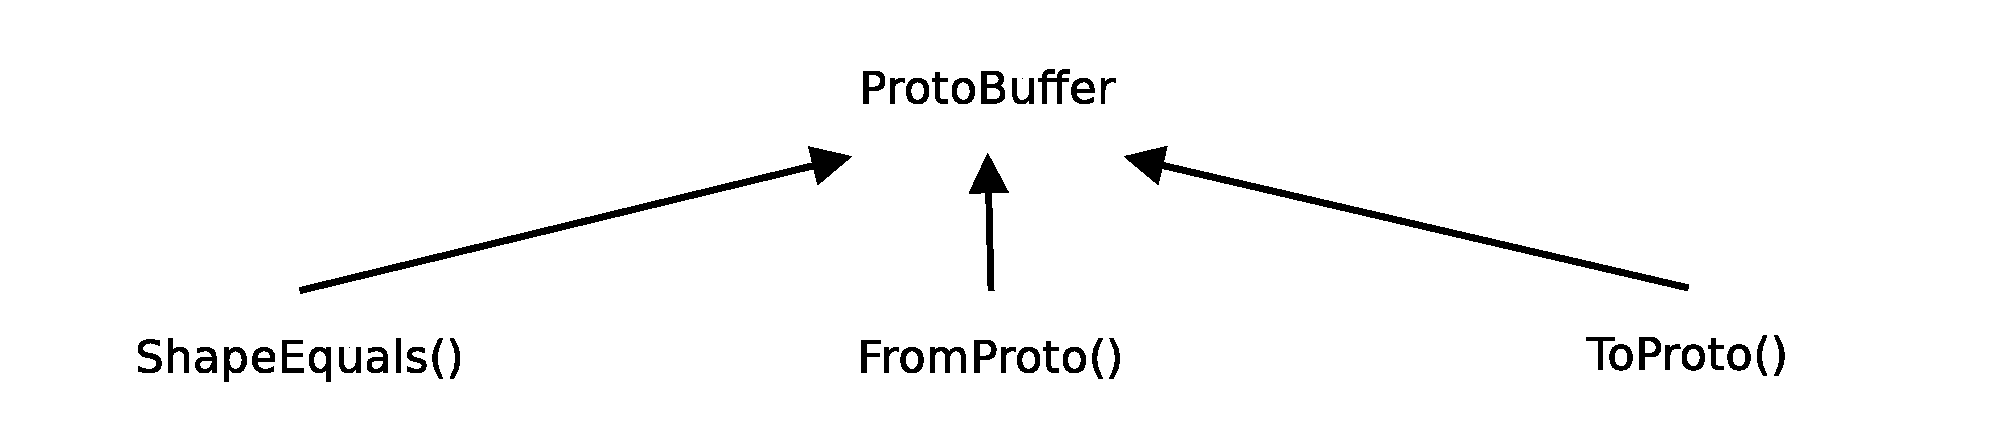
\includegraphics[height=3cm ,width=15cm,angle=0]{include/chp_blob_cls/figures/blob_architecture_proto.eps}
\end{cnfigure}